% Niveau :      PC
% Discipline :  Mécaflu
%Mots clés :    Ondes de surface

\begin{exercise}{\textit{Jeux de vagues}}{3}{Spé}
{Mécanique des fluides, Fluides parfaits, Tension superficielle}{bermu}

\begin{questions}
    \questioncours Décrire et comparer à l'aide d'un tableau comportant les différents paramètres que vous jugerez pertinents (\emph{e.g.} fréquence, impédance...) les phénomènes ondulatoires physiques que vous connaissez. On conservera ce tableau pour la suite de l'exercice. \label{que:ondes}
\begin{EnvUplevel}
Nous étudions par la suite un liquide dont la surface est libre d'osciller.
\begin{figure}[H]
    \centering
    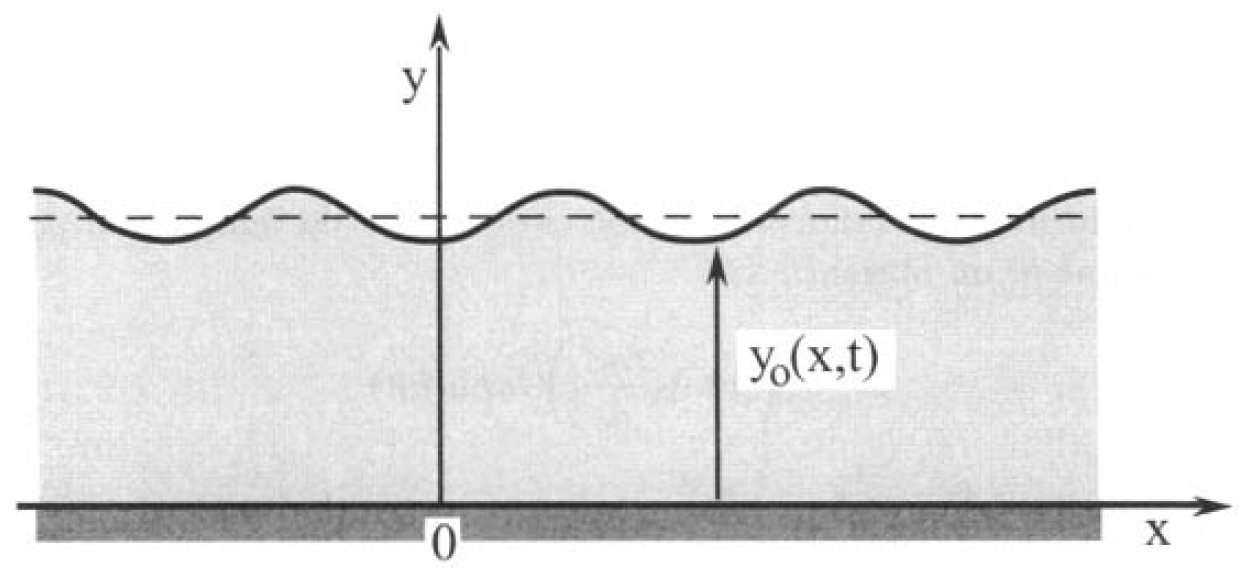
\includegraphics[width=0.5\linewidth]{mecaflu/barque.png}
    \vspace{-1.5em}
    \caption{Geometrie de la couche de liquide pour l'étude de la propagation
des ondes de surface.}
\end{figure}
Le liquide est de profondeur $h$. On supposera que les ondes sont de faible amplitude.
\end{EnvUplevel}
    \question Décrire les différents termes de l'équation d'Euler en 2D dans un champ de pesanteur $\vg$. Définir \emph{écoulement potentiel} et introduire le potentiel des vitesses $\Phi$.
    \question Montrer que dans notre cas l'équation d'Euler devient
    $$\pdv{\Phi}{t} + \dfrac{p}{\rho} + g y = \text{cte}.$$
    \question\label{que:laplace} En justifiant que l'écoulement est irrationnel et que le fluide est incompressible, montrez que $\Phi$ vérifie l'équation de Laplace.
    \question\label{que:inter} Donner les conditions aux limites pour $p$, $\Phi$ et $y_0$ en $y = y_0(x,t)$.
    \question\label{que:kelvin} En déduire que le potentiel $\Phi$ vérifie en $y = y_0(x,t)$ :
    $$\pdv[2]{\Phi}{t} + g\pdv{\Phi}{y} = 0.\vspace{-1.5em}$$
\uplevel{Nous allons à présent chercher des solutions sous forme d'onde de célérité $c$ : \  $\Phi(x,y,t) = \Phi_0 f(y) e^{ik(x-ct)}.$}
    \question Compte tenu de la question \ref{que:laplace}, donner l'expression de la fonction $f$.
    \question Déduire de la question \ref{que:kelvin} que la relation de dispersion des ondes de gravité est
    $$\omega^2 = gk\tanh(hk).$$
    Discuter de cette relation et des limites en eau peu profonde $h \ll \lambda$ et très profonde $h \gg \lambda$.
    \question Compléter le tableau de la question \ref{que:ondes} au vu de la question précédente.
\end{questions}
\plusloin[Les ondes gravito-capillaires]
La différence de pression $\Delta p$ à une interface liquide vapeur $y_0(x,t)$ ayant pour tension superficielle $\gamma$ est, pour une faible courbure de l'interface, donnée par la Loi de Laplace
$$\Delta p \simeq \gamma \pdv[2]{y_0}{x}.\vspace{-0.5em}$$
En revoyant le résultat de la question \ref{que:inter}, montrez que la relation de dispersion des ondes gravito-capillaires est\vspace*{-2ex}
$$\omega^2 = k^2 \ gh\qty(1 + \dfrac{\gamma }{\rho g}k^2)\dfrac{\tanh{kh}}{kh}.$$

\end{exercise}